%%%%%%%%%%%%%%%%%%%%%%% file template.tex %%%%%%%%%%%%%%%%%%%%%%%%%
%
% This is a general template file for the LaTeX package SVJour3
% for Springer journals.          Springer Heidelberg 2010/09/16
%
% Copy it to a new file with a new name and use it as the basis
% for your article. Delete % signs as needed.
%
% This template includes a few options for different layouts and
% content for various journals. Please consult a previous issue of
% your journal as needed.
%
%%%%%%%%%%%%%%%%%%%%%%%%%%%%%%%%%%%%%%%%%%%%%%%%%%%%%%%%%%%%%%%%%%%
%
% First comes an example EPS file -- just ignore it and
% proceed on the \documentclass line
% your LaTeX will extract the file if required
\begin{filecontents*}{example.eps}
%!PS-Adobe-3.0 EPSF-3.0
%%BoundingBox: 19 19 221 221
%%CreationDate: Mon Sep 29 1997
%%Creator: programmed by hand (JK)
%%EndComments
gsave
newpath
  20 20 moveto
  20 220 lineto
  220 220 lineto
  220 20 lineto
closepath
2 setlinewidth
gsave
  .4 setgray fill
grestore
stroke
grestore
\end{filecontents*}
%
\RequirePackage{fix-cm}
%
%\documentclass{svjour3}                     % onecolumn (standard format)
%\documentclass[smallcondensed]{svjour3}     % onecolumn (ditto)
%\documentclass[smallextended]{svjour3}       % onecolumn (second format)
\documentclass[twocolumn]{svjour3}          % twocolumn
%
\smartqed  % flush right qed marks, e.g. at end of proof
%
\usepackage{graphicx}
%
% \usepackage{mathptmx}      % use Times fonts if available on your TeX system
%
\usepackage{url}
% insert here the call for the packages your document requires
%\usepackage{latexsym}
% etc.
%
% please place your own definitions here and don't use \def but
% \newcommand{}{}
%
% Insert the name of "your journal" with
% \journalname{myjournal}
%
\begin{document}

\title{Dynamic Virtualized Deployment of Particle Physics Environments on a
  High-Performance Computing Cluster%\thanks{Grants or other notes
%about the article that should go on the front page should be
%placed here. General acknowledgments should be placed at the end of the article.}
}
%\subtitle{Do you have a subtitle?\\ If so, write it here}

%\titlerunning{Short form of title}        % if too long for running head

\author{Felix B\"uhrer \and Anton Gamel  \and Michael Janczyk \and
  Markus Schumacher \and
  Ulrike Schnoor \and Bernd Wiebelt \and People from KIT
  % etc.
}

%\authorrunning{Short form of author list} % if too long for running head

\institute{U. Schnoor \at
              CERN \\
              \email{ulrike.schnoor@cern.ch}           %  \\
%             \emph{Present address:} of F. Author  %  if needed
           \and
           F. B\"uhrer \at
              Universit\"at Freiburg
}

\date{Received: date / Accepted: date}
% The correct dates will be entered by the editor


\maketitle

\begin{abstract}
Particle Physics experiments at the Large Hadron Collider (LHC) need a high
amount of computing resources for data processing, simulation, and analysis.
High-Performance Computing (HPC) resources provided by universities
can be useful supplements to the existing World-wide LHC Computing Grid resources
allocated by the collaboration. At the university of Frei\-burg, the
shared HPC cluster "NEMO" has been made available to ATLAS and CMS
users accessing NEMO from external collaboration-specific resources.
 To this effect, the full environment corresponding to a WLCG center
 is provided. The interplay between the NEMO and the external
 resources' schedulers is ensured through the ROCED service.
An OpenStack infrastructure is deployed at NEMO to orchestrate the
simultaneous usage for bare metal and virtualized jobs.
Through the setup, resources are provided to users in an automatized,
on-demand way. The performance of the virtualized environment has been
evaluated for particle physics jobs.

%Insert your abstract here. Include keywords, PACS and mathematical
%subject classification numbers as needed.
\keywords{Virtualization \and Particle Physics \and Grid Computing \and More keywords}
% \PACS{PACS code1 \and PACS code2 \and more}
% \subclass{MSC code1 \and MSC code2 \and more}
\end{abstract}




\section{Introduction}
\label{intro}

This paper presents the concepts and implementation of providing a HPC
resource to ATLAS and CMS users accessing external clusters connected
to the World-wide computing grid (WLCG) with the purpose of running
data production as well as data analysis on the HPC host system.
For this purpose, the HPC cluster NEMO at the University of Freiburg
is deploying an OpenStack instance to handle the virtual machines.
The schedulers on the NEMO and the external resources are connected
through the ROCED service\cite{ROCED}.



\section{Virtualization infrastructure}
\label{sec:openstack}
$\to$Rechenzentrum\\
\textit{Motivation for virtualized approach (increase the number of potential
user groups without increasing the administrative effort); virtualized
research environments; description of infrastructure for virtualized research environments
(OpenStack, startVM etc) on NEMO }

The computer center of the University of Freiburg provides reasonably scaled research
infrastructures like cloud, storage and especially HPC to cater to the needs of various
scientific communities. To operate systems comprised of more than 1000 inidividual nodes
with a small group significant standardization in hardware and software is necessary. To
address the particular needs of individual scientific communities and research groups the
computer is participating in a state-wide HPC federation and cooperating with other
computer centers within the bwHPC-C5 project. The bwForCluster NEMO is focusing on the
domains of neuroscience, microsystems technology and particle physics, offering its
services to all reasearchers of these fields working at one of the nine Baden-Wuerttemberg
universities. The level of granularity of the software stack provided is not fine enough to
directly support the quite special requirements of world-wide efforts like the ATLAS or CMS
experiments. To utilize the system optimally and open the cluster to as many different
needs as possible without overstretching its own man power novel approaches were
necessary. Thus, the eScience group pooled in it's expertise in cloud operation especially
the use of OpenStack as a cloud platform to provide a more flexible software deployment
on the cluster beside the existing module system.

The state sponsored E-Research-Initiative on virtualized research environments (VREs)
provided the perfect environment to bring together both the infrastructure providers like
the computer center and selected research communities e.g. in the two year ViCE project.
The CMS and ATLAS groups cooperate in this project or as a bwHPC-C5 tiger team to tackle
the particular challenges of VREs like provisioning, setup, scheduling and decommissioning.
A VRE in the context of this paper is a complete software stack as it would get installed on a
compute cluster fitted to ATLAS or CMS groups demand. The resulting filesystem is a
container presented as a single file. From the computer center's perspective this container
is seen as a black box requiring no involvement or efforts. From the researchers
perspective the VRE is an individual (virtual) server where everything from the hardware --
at least to a certain degree like CPU or RAM dimensioning -- up to the operating system,
applications and configurations can be controlled solely by the research groups.
To allow more flexible software environments the standard bare metal operation the NEMO
cluster got extended with a parallel installation of OpenStack components \cite{hpc-symp:2016}. They are getting orchestrated from a special management node which
provides the necessary interfaces to the other services. The NEMO cluster as it's siblings
throughout the state use Adaptive's MOAB as a scheduler of compute jobs. To allow
seemless coexistence of both bare metal and virtualied jobs the scheduler has to handle
both of them. As the scheduler does not look into the VRE virtual machines, it cannot assess
if they are actually active or idle. To solve this, a customized glue component got introduced
(to be described in further detail in section XX). The virtual machines started and stopped bythe OpenStack nova(?) components triggered by ??. 

$<$Michael, hier wollen wir evtl. noch etwas mehr dazu sagen!?$>$

\section{Generation of the image}
The research environments in the use case described in this paper are OpenStack containers in the
format of compatible VM images.
These images are provided in an automatized
way allowing versioning and archiving of the environments captured in
the images. The approaches used in the
different groups are described in the following.

\subsection{Packer combined with Puppet}
$\to$ATLAS Freiburg\\

One approach to generating the image is the open-source tool
\texttt{packer}\cite{packer}, interfaced to \texttt{puppet}\cite{puppet}.
\texttt{packer} allows to configure an image based on an \texttt{.iso} file using a kickstart [ref] fine and flexible script-based configuration. 
It also provides an interface to \texttt{puppet} making it a convenient tool if an existing \texttt{puppet} role is to be used for the images. If the roles are defined according to the hostname of the machine as is conventional in \texttt{puppet} with \texttt{hieradata}, the hostname needs to be set in the scripts supplied to \texttt{packer}. Propagation of certificates require an initial manual start of a machine with the same hostname to allow handshake signing of the certificate from the \texttt{puppet} server.

\textit{setting hostname to get correct role from puppet; puppet certificates; anything else? }



\subsection{Image generation using the Oz toolkit}
%$\to$CMS Karlsruhe\\
Another option to employ a fully-automated procedure is to use the OZ toolkit~\cite{OZ}. All requirements and configuration options of an image can be specified via an XML file, called template. The partitioning and installation process of the operating system is fully automated, as OZ will use the remote-control capabilities of the local hypervisor. After the installation of the operating system, additional libraries and configuration files can be installed. Once the image has been built, it is automatically compressed and uploaded to a remote cloud site.
Using this technique allows to build images in a reproducible fashion, as all templated files are version controlled using git. Furthermore, existing template files are easy to adapt to new sites and experiment configurations.

\section{Interfacing the schedulers using ROCED}
Introduction about the requirements for an in-between layer
\\$\to $ Karlsruhe
\subsection{ROCED}
\begin{figure*}
\begin{center}
  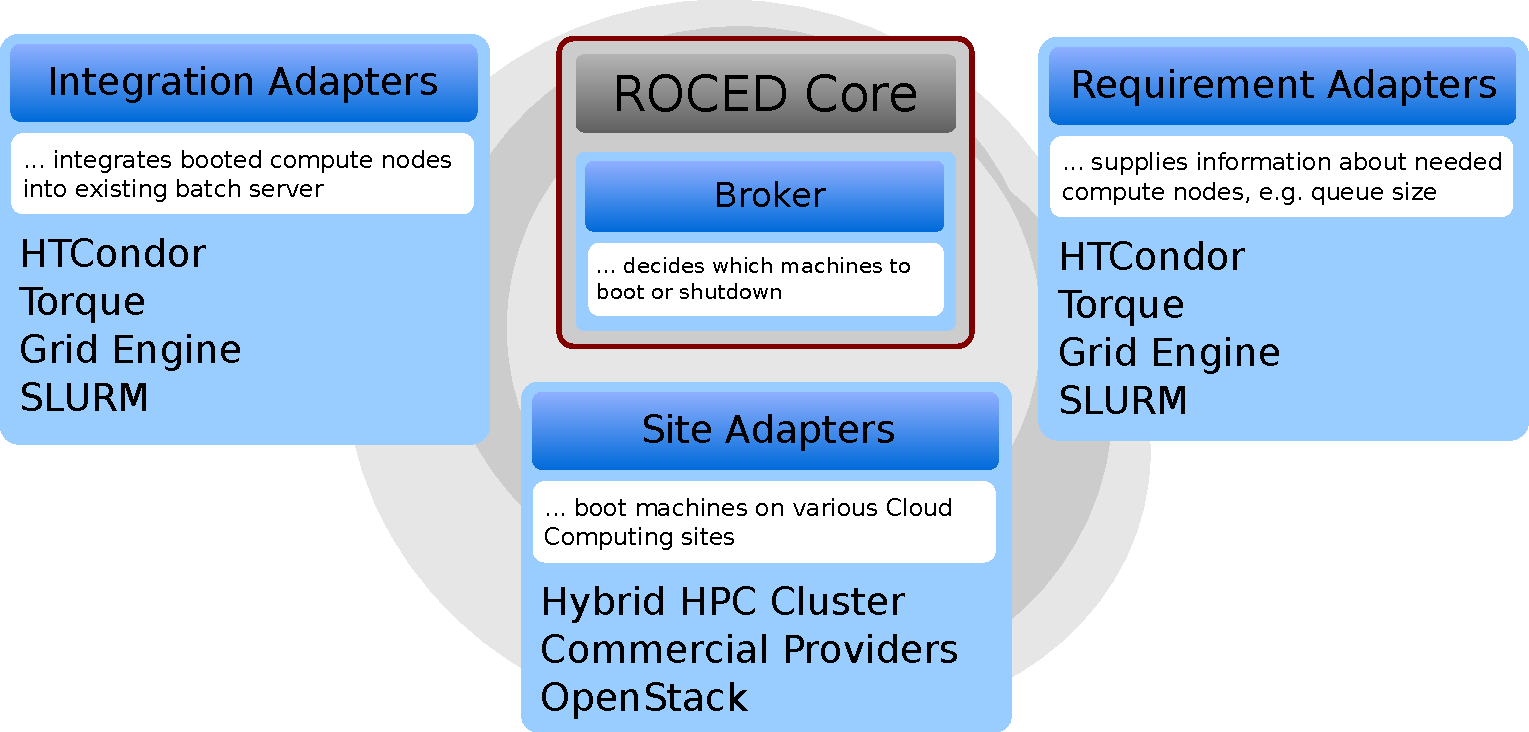
\includegraphics[width=0.9\linewidth]{figures/roced_design_flat.pdf}
  \caption{Overview of the ROCED modular design. The ROCED Core contains the Broker which decides when and on which sites new virtual machines are booted. The Requirement Adapters report about the utilization and resource requirements of the attached batch systems. The Site Adapter is responsible to manage the lifetime of virtual machines on an cloud site and the Integration Adapter ensure that newly booted machines are integrated into the batch system.}
  \label{fig-frplots}
\end{center}
\end{figure*}

%$\to$ CMS Karlsruhe
The cloud meta-scheduler ROCED (Responsive On-demand Cloud Enabled Deployment) has been developed at the KIT since 2010~\cite{ROCED}. ROCED is written in a modular
fashion and the interfaces to batch systems and cloud sites are implemented as so-called \textit{Adapters}. This makes ROCED independent of a specific user group or workflow. It provides a scheduling core which collects the current requirement of computing resources and decides if virtual machines need to be started or can be stopped. One or more Requirement Adapters report the current queue status of batch systems to the central scheduling core. Currently, Requirement Adapters are implemented for the Slurm, Torque, HTCondor and GridEngine batch systems. The Site Adapters allow ROCED to start, stop and monitor virtual machines on multiple cloud sites. Implementations exist for Amazon EC2, OpenStack, OpenNebula and Maob-based virtualization at HPC centers. Special care has been put into the resilience of ROCED: it can automatically terminate non-responsive machines and restart virtual machines in case some machines dropped out. This allows VM setups orchestrated by ROCED with thousands of virtual machines and many tens of thousands of jobs to run in production environments.


\subsection{Using HTCondor as front-end scheduler}\label{sec:ROCED:HTCondor}
%$\to$ CMS Karlsruhe
The open-source HTCondor project provides a workload management system which is highly configurable and modular~\cite{HTCondor}. Batch processing workflows can be submitted and are then forwarded by HTCondor to idle resources. HTCondor maintains a resource pool, which worker nodes in a local or remote cluster can join. Once HTCondor has verified the authenticity and features of the newly joined machines, computing jobs are automatically transferred. Special features to connect from within isolated network zones, for example via a NAT-Portal, to the central HTCondor pool are available. The Connection Brokering (CCB) service is especially valuable to connect virtual machines to the central pool. These features and the well-known ability of HTCondor to scale to O(100k) of parallel batch jobs lets us decide to use HTCondor as a workload management system.

The virtual machines spawned for the CMS user group of the KIT come with the HTCondor client (\texttt{startd}) pre-installed and this client is started after the machine has fully booted and connects to the central HTCondor pool at the KIT via a shared secret. Due to HTCondor's dynamic design, new machines in the pool will automatically receive jobs and the transfer of the job configuration and meta-data files is handled via HTCondor's internal file transfer systems.

\subsection{Using SLURM as front-end scheduler}
$\to$ ATLAS Freiburg\\
Alternatively to the approach in Sec.~\ref{sec:ROCED:HTCondor}, the
scheduler \textsc{Slurm} has been incorporated into the ROCED setup by
a group at University of Freiburg.
While \textsc{Slurm} provides a built-in functionality for dynamic
startup of resources in the \textit{Slurm Elastic Computing} module\cite{SlurmElastic}. 
However, this is not suitable for resources which are not
expected to be available nearly instantaneously, in this case due to
the presence of a queue in the host system which may postpone the start
of a resource by a significant, varying period.
In addition, the transfer of information from one scheduler the the
other, and therefore to the user, is very limited.
Therefore, ROCED has been chosen as the interface between the
\textsc{Moab} scheduler on the host system and the \textsc{Slurm}
scheduler on the submission side.

For \textsc{Slurm}, it is necessary that each potential virtual
machine is registered in the configuration at the time of start of the
slurm server as well as the client. \textsc{Slurm} configurations also
need to be in agreement between server and client.
Therefore, a range of hostnames is registered in the configuration in
a way that is mapped to potential IP addresses of virtual machines.
These virtual machines have a fixed number of CPUs and memory and are
registered under a certain partition.
When a job is submitted to this partition and no other resource is
available, information from the \textsc{Slurm} \texttt{squeue} and
\texttt{sinfo} commands is requested and parsed in such a way to
obtain the amount of requested information.

Since the ATLAS Freiburg group comprises three sub-groups, each mapped
to a different account on \textsc{Moab}/ NEMO, special care is taken to
avoid interference of resources used by another account, while
allowing jobs from one group to occupy otherwise idle resources of another group.


ROCED determines the amount of VMs to be started and sends the
corresponding startVM commands to \textsc{Moab}.
After the virtual machine has booted, the hostname is set to the IP
dependent name which is known to the \textsc{Slurm} configuration.
A cron job executes a few sanity
checks on the system.
Upon successful execution of these tests, the \textsc{Slurm} client
running in the VM starts accepting the queued jobs.
After completion of the jobs and a certain period of being idle, the
\textsc{Slurm} client in the machine drains itself and the machine
shuts itself down.
The IP address as well as the corresponding hostname in \textsc{Slurm}
are then released and can be used again.







\section{Analysis of performance and usage}

The approach described so far has been implemented and put into
production in the research groups at University of Freiburg
(Physikalisches Institut) and Karlsruhe (... Institut).
The following chapter presents statistical results of the analysis of
the performance of the virtualized setup both in terms of job
performance as well as usage statistics.


\subsection{HEPSPEC benchmarks}
$\to$ ATLAS Freiburg\\
The HEPSPEC ........ allow standardized benchmarking of CPU
performance ......

For an estimate of the performance of the virtual machines, machines
with the same hardware configuration are compared which are either
deployed via the existing Tier2/3 boot system (``bare metal'') or via the NEMO
OpenStack in virtual machines.

The results of the HEPSPEC benchmarks are presented in
Fig.~\ref{fig:HEPSPECpCPUvsCPU-atlas} which shows the HEPSPEC score
determined per number of CPUs versus the number of CPUs.
Different tests have been performed \textit{bare metal}, where the
benchmark code is run either with user rights (``realistic load'') or
with root privileges (``machine reserved'').
The results illustrate that the bare-metal jobs are less performant
than those performed in virtual machines on NEMO with machines under
realistic load. Tests carried out
in user space on the virtual machines are approaching \textit{bare metal} tests with
root permissions.


\begin{figure}[htbp]
%% For example, with the graphicx package use
  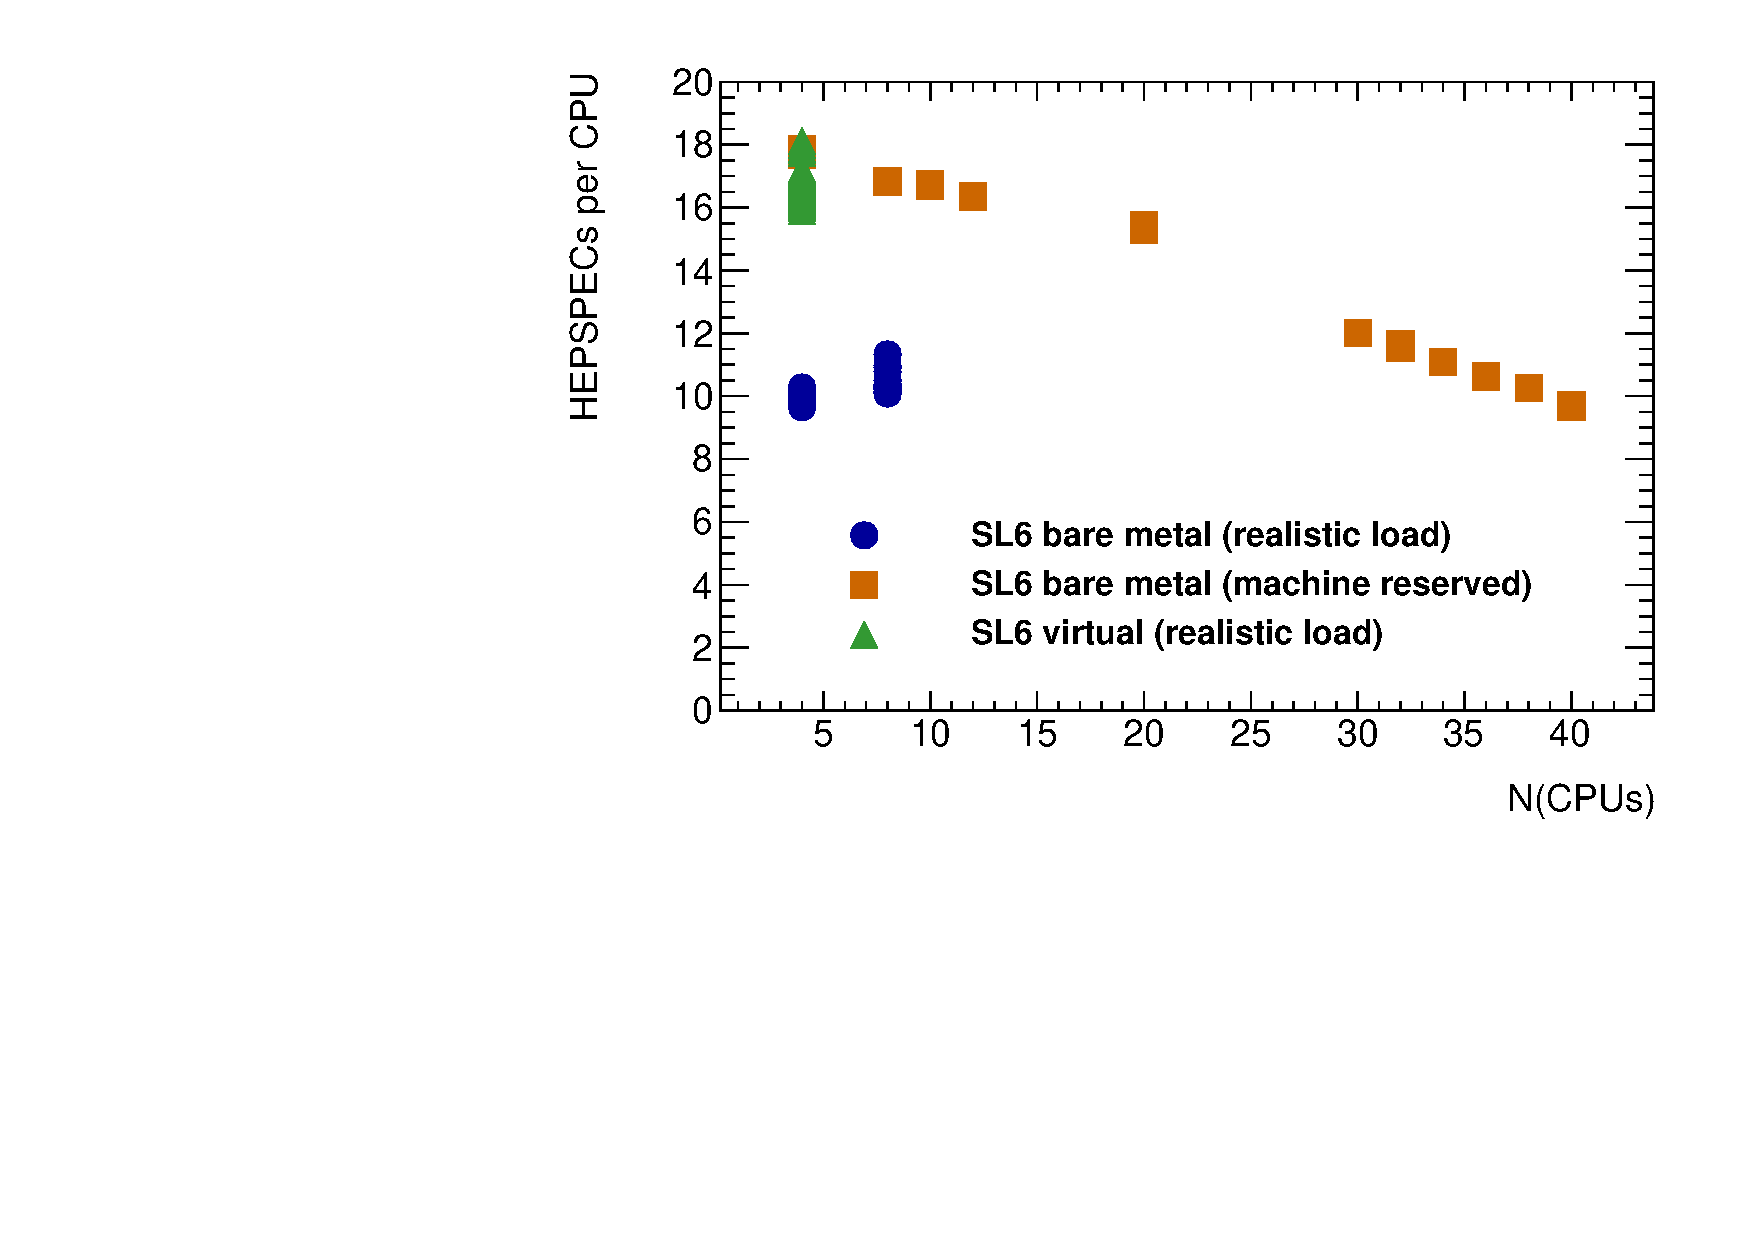
\includegraphics[width=\columnwidth]{figures/HEPSPECpCPUvsCPU.pdf}
\caption{Results of HEPSPEC benchmark tests: HEPSPEC per number of
  CPUs in dependence of number of CPUs.}
\label{fig:HEPSPECpCPUvsCPU-atlas}
\end{figure}

As it is expected from first principles that the virtualisation
reduces the CPU power available to the process, these results indicate
non-optimal configuration of the bare-metal running. However it is
reassuring for the use-case of running in the ATLAS environment on
NEMO that the performance does not suffer.



%
%realistic load: as user
%machine reserved: root
%Hier sieht man, dass die Bare-Metal-User-Jobs wesentlich weniger performant sind, und die User-Jobs auf den VMs beinahe an die ROOT-Tests auf bare-metal herankommen. Interessant ist auch, dass bei den User-Jobs der Trend umgekehrt ist: Dort ist die HEPSPEC pro Core(!) etwas besser fuer 8 Cores. Es koennte aber auch sein, dass das bei den ROOT-Jobs auch so waere, dort haben wir die Zahlen in dem Bereich ja nicht.
%



\subsection{Production of simulation data}
$\to$ATLAS Freiburg
\\As a realistic job which could be run by ATLAS users on the NEMO
cluster, the production of simulated events with the Monte Carlo
generators PowhegBox and Pythia8 has been executed in the virtual
machines.
These jobs do not constitute the best-case scenario but rather
realistic conditions from the point of view of the user.

\subsection{Data analysis}
$\to$ATLAS Freiburg 

\subsection{Usage statistics}
Figure \ref{fig-frplots} show the utilization of virtual machines which were orchestraded by ROCED depending on the resource demands of the users of the KIT group. At peak times, up to 9000 virtual cores were filled with user jobs, which is more than half of the 16.000 cores of the NEMO cluster. 

\begin{figure}
\begin{center}
  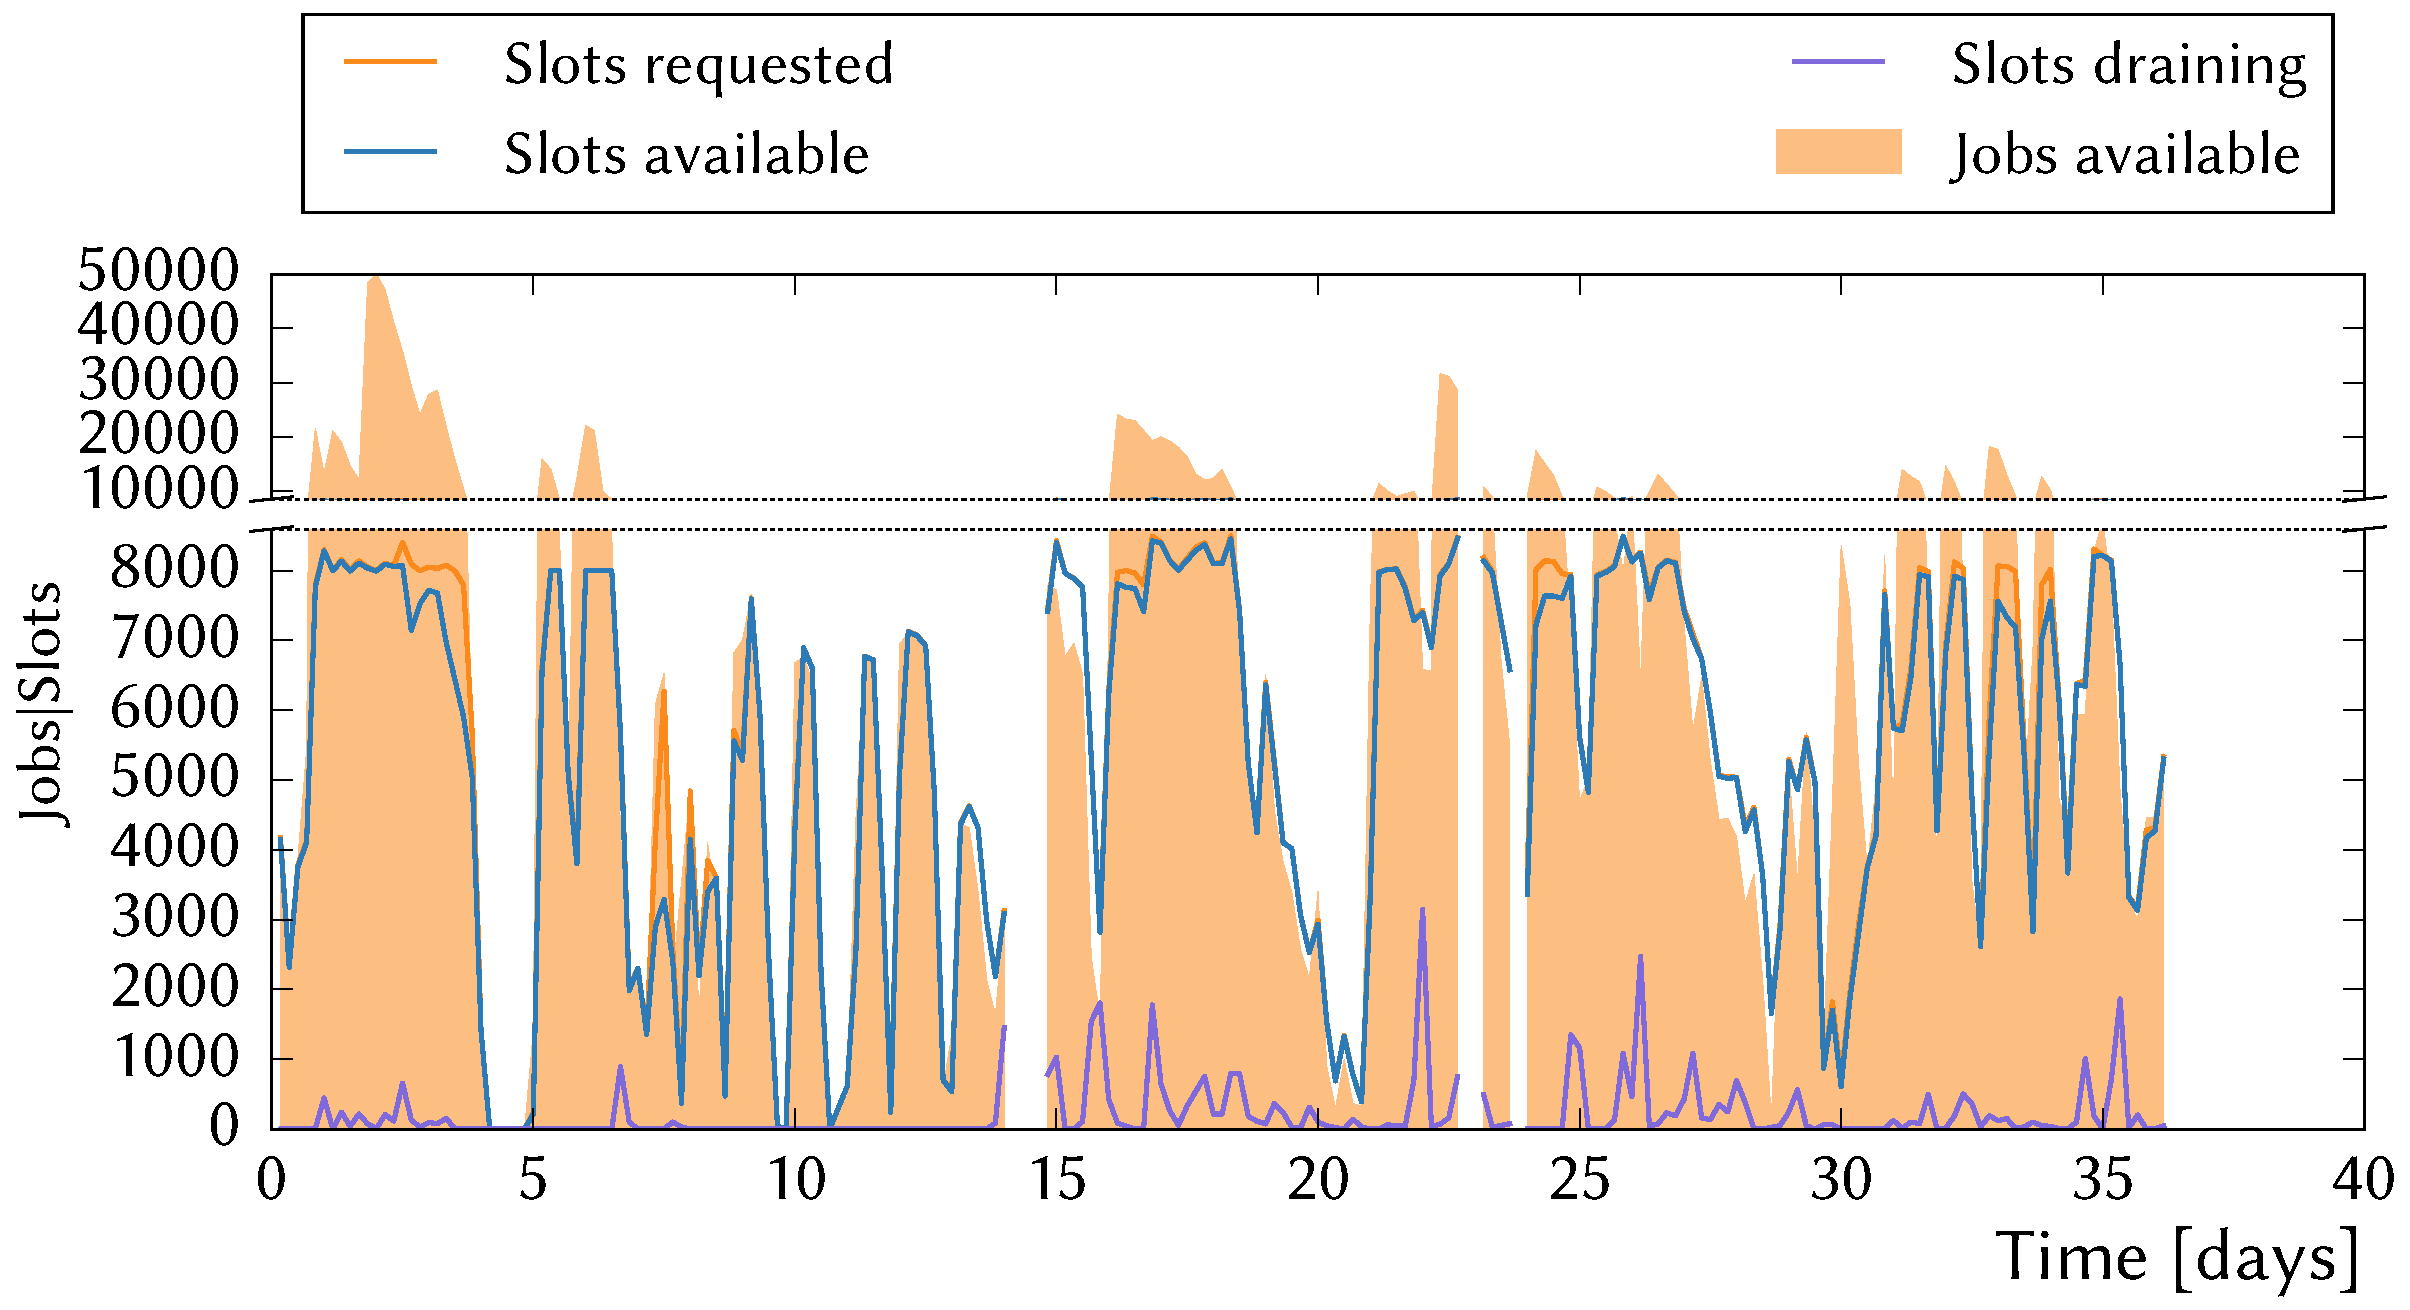
\includegraphics[width=0.9\linewidth]{figures/NEMO_KIT_utiliztion.pdf}
  \caption{Utilization of the shared HPC system by booted virtual machines. Up to 9000 virtual cores were in use at peak times. The fluctuations in the utilization reflects the patterns of the submission of jobs by our institute users. The number of draining slots displays the amount of job slots still processing jobs while the rest of the node's slot are already empty.}
  \label{fig-frplots}
\end{center}
\end{figure}


\section{Conclusions and Outlook}




A system for the dynamic, on-demand provisioning of virtual machines
to run jobs in a High-Energy Physics context on an external, not
dedicated resource as realized at the HPC
cluster ``NEMO'' at University of Freiburg has been described. 
Reasons for the need for an interface between the schedulers of the host system
and the external system from which requests are sent have been
explained. 
The performance and usage have been analyzed for two groups. 

This approach can be generalized to other platforms and possibly also
other forms of virtualized environments (containers).


Using virtualization inside an HPC system opens up the possibilities for several interesting
features. While their implementation would require tighter integration between HPC
scheduler
and virtualization framework, they could solve several classic problems with HPC systems,
especially those designated for novice HPC users.
Snapshot and migration functionality for running virtual machine instances are a typical
feature of virtualization frameworks. This means that running processes can be stopped,
possibly
moved to a different node in the virtualization cluster and then resumed. For an HPC
system,
this would be practical for two use cases. The first one concerns long running monolithic
jobs.
These are, for very practical reasons, non favored jobs in HPC environments, assuming they
are permitted in the first place. However, the costs to adapt a particular workflow based on
such monolithic tasks to a HPC system, e.g. by parallelizing and partitioning it manually,
may sometimes exceed the practical use of the resulting solution. If the monolithic job
could
automatically be stopped, checkpointed and resumed at regular intervals, this might very
well
constitute a more economic procedure. In the second use case, if there is a mix of
pleasingly
parallel high throughput jobs (using only single cores or nodes) and massively parallel high
performance jobs (using several nodes), the second class of jobs should be concentrated on
nodes that share optimal high performance network communication paths. Typically this is
accomplished by high investments in the network topology or
sophisticated tuning of the
job
queue. However, if jobs could be moved around the physical machines (i.e. ”de
fragmented”),
optimal high performance network communication paths can be guaranteed by
concentrating
massively parallel jobs on the same or adjacent high performance network switches.



A system for the dynamic, on-demand provisioning of virtual machines
to run jobs in a High-Energy Physics context on an external, not
dedicated resource as realized at the HPC
cluster ``NEMO'' at University of Freiburg has been described. 
Reasons for the need for an interface between the schedulers of the host system
and the external system from which requests are sent have been
explained. 
The performance and usage have been analyzed for two groups. 

This approach can be generalized to other platforms and possibly also
other forms of virtualized environments (containers).
















%\subsection{Subsection title}
%\label{sec:2}
%as required. Don't forget to give each section
%and subsection a unique label (see Sect.~\ref{sec:1}).

%\paragraph{Paragraph headings} Use paragraph headings as needed.
%\begin{equation}
%a^2+b^2=c^2
%\end{equation}
%
%% For one-column wide figures use
%\begin{figure}
%% Use the relevant command to insert your figure file.
%% For example, with the graphicx package use
%  \includegraphics{example.eps}
%% figure caption is below the figure
%\caption{Please write your figure caption here}
%\label{fig:1}       % Give a unique label
%\end{figure}
%%
%% For two-column wide figures use
%\begin{figure*}
%% Use the relevant command to insert your figure file.
%% For example, with the graphicx package use
%  \includegraphics[width=0.75\textwidth]{example.eps}
%% figure caption is below the figure
%\caption{Please write your figure caption here}
%\label{fig:2}       % Give a unique label
%\end{figure*}
%
%% For tables use
%\begin{table}
%% table caption is above the table
%\caption{Please write your table caption here}
%\label{tab:1}       % Give a unique label
%% For LaTeX tables use
%\begin{tabular}{lll}
%\hline\noalign{\smallskip}
%first & second & third  \\
%\noalign{\smallskip}\hline\noalign{\smallskip}
%number & number & number \\
%number & number & number \\
%\noalign{\smallskip}\hline
%\end{tabular}
%\end{table}


%\begin{acknowledgements}
%If you'd like to thank anyone, place your comments here
%and remove the percent signs.
%\end{acknowledgements}

% BibTeX users please use one of
%\bibliographystyle{spbasic}      % basic style, author-year citations
%\bibliographystyle{spmpsci}      % mathematics and physical sciences
%\bibliographystyle{spphys}       % APS-like style for physics
%\bibliography{}   % name your BibTeX data base

% Non-BibTeX users please use
\begin{thebibliography}{}
%
% and use \bibitem to create references. Consult the Instructions
% for authors for reference list style.
%
\bibitem{Openstack}
OpenStack Open Source Cloud Computing Software
\url{https://www.openstack.org/}, accessed 2017-01-10

\bibitem{ROCED}
ROCED Cloud Meta-Scheduler project website
\url{https://github.com/roced-scheduler/ROCED}, accessed 2017-01-10

\bibitem{OZ}
Oz image generation toolkit
\url{https://github.com/clalancette/oz}, accessed 2017-01-10

\bibitem{HTCondor}
HTCondor workload manager
\url{https://research.cs.wisc.edu/htcondor/}, accessed 2017-01-10

\bibitem{packer}

Packer: tool for creating machine and container images for multiple platforms from a single source configuration. 
\url{https://www.packer.io/}, accessed 2017-01-13

\bibitem{puppet}

Puppet Enterprise. ``IT automation for cloud, security, and DevOps.''
\url{https://puppet.com/}, accessed 2017-01-10

\bibitem{SlurmElastic}
Slurm Elastic Computing ....


\bibitem{hpc-symp:2016}
Dirk von Suchodoletz, Bernd Wiebelt, Konrad Meier,Michael Janczyk,
  Flexible HPC: bwForCluster NEMO, 
Proceedings of the 3rd bwHPC-Symposium: Heidelberg 2016, \url{http://books.ub.uni
heidelberg.de/heibooks/reader/download/308/308-4-79237-1-10-20171002.pdf}

%title={Flexible HPC: bwForCluster NEMO},
%authors={Dirk von Suchodoletz and Bernd Wiebelt and Konrad Meier and
%Michael Janczyk},
%editors={Richling, Sabine and Baumann, Martin and Heuveline, Vincent},
%booktitle={Proceedings of the 3rd bwHPC-Symposium: Heidelberg 2016},
%publisher={heiBOOKS},
%year={2017},
%DOI={10.11588/heibooks.308.418},
%url={http://books.ub.uni
%heidelberg.de/heibooks/reader/download/308/308-4-79237-1-10-20171002.pdf}
%}

%\bibitem{RefJ}
% Format for Journal Reference
%Author, Article title, Journal, Volume, page numbers (year)
% Format for books
%\bibitem{RefB}
%Author, Book title, page numbers. Publisher, place (year)
% etc
\end{thebibliography}

\end{document}
% end of file template.tex

